\subsubsection{Power and Safety Tests}

\paragraph{Rail Voltage Verification}

All power rails were measured under normal operating conditions using an OWON XDM1241 multimeter.
Table~\ref{tab:rail-voltages} summarises the measured values against their expected levels.

\begin{table}[H]
    \centering
    \begin{tabular}{llll}
        \toprule
        \textbf{Rail} & \textbf{Source} & \textbf{Expected} & \textbf{Measured} \\
        \midrule
        $+\SI{5}{\volt}$   & Buck converter from $+\SI{12}{\volt}$ bus & $\SI{5.00}{\volt}$ & $\SI{5.00}{\volt}$ \\
        $+\SI{3.3}{\volt}$ & LDO from $+\SI{5}{\volt}$                 & $\SI{3.30}{\volt}$ & $\SI{3.29}{\volt}$ \\
        \bottomrule
    \end{tabular}
    \caption{Derived power rail voltages measured under normal operating conditions.}
    \label{tab:rail-voltages}
\end{table}

Both derived rails are in close deviation of their target values, confirming correct operation of the buck converter and LDO.
The Eurorack bus rails ($+\SI{12}{\volt}$ and $-\SI{12}{\volt}$) were supplied by a linear lab power supply with current readings. The power behaviour in a host case with its own power supply were not independently measured.

\paragraph{Current Consumption}

The firmware executes the full DSP chain --- tape player, exciter, and Schroeder reverb --- unconditionally on every audio block at \qty{48}{\kilo\hertz}, regardless of whether audio is recorded in the buffer.
There is therefore no meaningful idle state; the current figures below represent steady-state operation.

Current draw was measured on the $+\SI{12}{\volt}$ and $-\SI{12}{\volt}$ Eurorack bus rails using the current display of an QJ3005E III bench supply, under two LED conditions.
The $+\SI{12}{\volt}$ rail supplies the LDO (\qty{3.3}{\volt} for MCU and analog circuitry) and the buck converter (\qty{5}{\volt} for WS2812 LEDs); the $-\SI{12}{\volt}$ rail supplies the op-amp negative rails exclusively.
The firmware caps WS2812 brightness at 170 out of 255 (\qty{67}{\percent}) because maximum brightness was too harsh too look at.

\begin{table}[H]
    \centering
    \begin{tabular}{lcc}
        \toprule
        \textbf{Condition} & \textbf{$+\SI{12}{\volt}$ (mA)} & \textbf{$-\SI{12}{\volt}$ (mA)} \\
        \midrule
        DSP active, LEDs off                                   & 80  & 20 \\
        DSP active, all 4 LEDs white at firmware max (170/255) & 120 & 20 \\
        Estimated worst case (all LEDs white at 255/255)       & $\approx 140$ & 20 \\
        \bottomrule
    \end{tabular}
    \caption{Current consumption on Eurorack bus rails. Worst-case estimate scales the measured LED contribution linearly: $\Delta I_\text{LED} = \SI{40}{\milli\ampere} \times \frac{255}{170} \approx \SI{60}{\milli\ampere}$.}
    \label{tab:power-consumption}
\end{table}

The $-\SI{12}{\volt}$ draw is constant across both conditions, as expected, since the op-amp stages are unaffected by LED state.
The LED contribution of \qty{40}{\milli\ampere} at firmware maximum brightness is consistent with four WS2812 LEDs at partial drive (\qty{10}{\milli\ampere} per LED).

\paragraph{Input Protection}

Input overvoltage protection is verified by design and confirmed through in-system testing at full Eurorack signal levels.
Gate inputs are clamped via transistor stages (EC-02); CV inputs use rail-guarded op-amp stages that limit the voltage presented to the STM32H7 ADC (EC-01, EC-02); audio inputs are attenuated by a passive resistor divider and clamped by a BAT54S dual Schottky diode to the codec supply rails (EC-03).
No input damage or anomalous behaviour was observed during extended operation with Eurorack-level signals.
The audio input protection is further verified by the loopback measurements in Section~\ref{sec:loopback-signal-level-measaurements}, which confirm correct ADC signal levels at \SI{10}{\volt_{pp}} input.

\subsubsection{Loopback and Signal Level Measurements}
\label{sec:loopback-signal-level-measaurements}

\paragraph{Measurement Setup}

To evaluate the audio signal path including analog frontents and AD/DA conversion, a sine was applied to 
the analog input at frequencies of \SI{100}{Hz}, \SI{1}{kHz}, and 
\qty{10}{kHz}. All test signals were applied at \SI{10}{V_{pp}}, corresponding to the standard Eurorack signal level. 
Input and output signals were captured simultaneously on a two-channel oscilloscope to verify signal integrity through the analog frontend and codec stages. 
To characterise the digital headroom, the DMA RX and TX buffers were read out via SWD during signal playback and plotted alongside the oscilloscope captures.

\paragraph{Results}

Figure~\ref{fig:loopback_scope} shows oscilloscope captures of the analog input (yellow) and output (blue) for a \SI{10}{V_{pp}} sine wave at \qty{100}{Hz} and \qty{1}{kHz}.

\begin{figure}[H]
	\centering
	\begin{minipage}{0.48\textwidth}
			\centering
			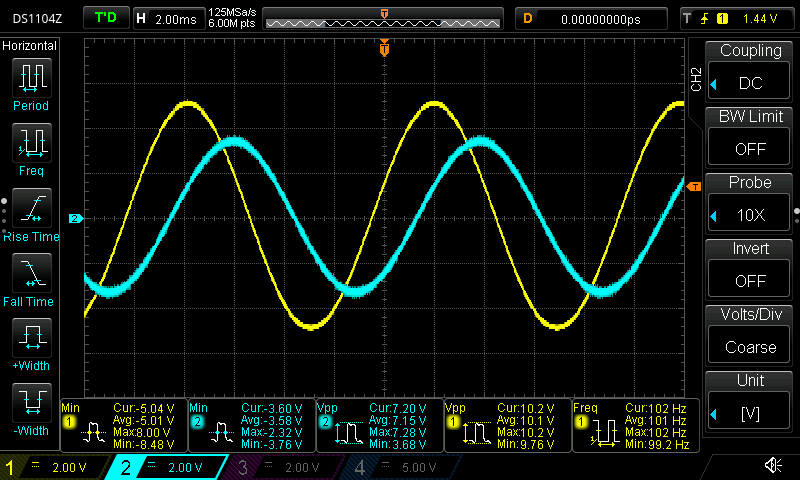
\includegraphics[width=\textwidth]{../images/signal_tests/codec_loopback/scope_loopback_fw-gain-1_10Vpp_sine_100Hz.png}
			\subcaption{\qty{100}{Hz} -- output \qty{7.20}{V_{pp}}}
		\end{minipage}
	\begin{minipage}{0.48\textwidth}
		\centering
		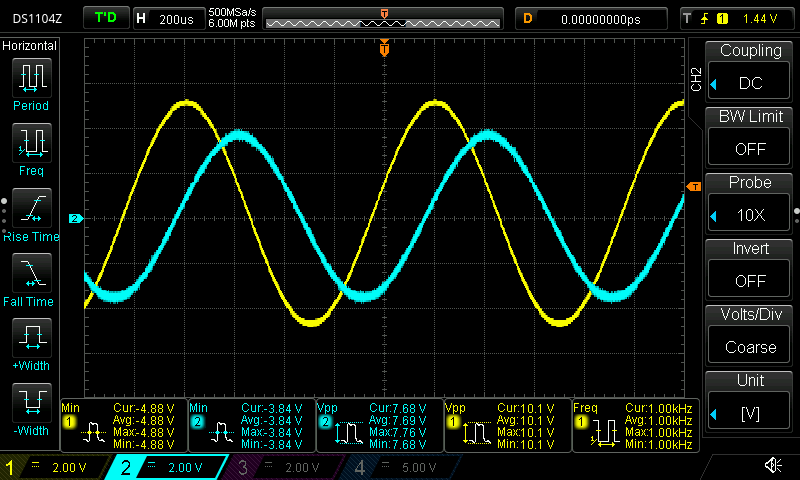
\includegraphics[width=\textwidth]{../images/signal_tests/codec_loopback/scope_loopback_fw-gain-1_10Vpp_sine_1kHz.png}
		\subcaption{\qty{1}{kHz} -- output \qty{7.68}{V_{pp}}}
	\end{minipage}
	\hfill

	\caption{Oscilloscope captures -- \SI{10}{V_{pp}} sine wave loopback at \SI{40}{\kilo\ohm} codec input impedance.}
	\label{fig:loopback_scope}
\end{figure}

Figure~\ref{fig:loopback_buf} shows the corresponding digitised RX and TX (half-)buffer
contents at \qty{1}{kHz} test signal.

\begin{figure}[H]
	\centering
	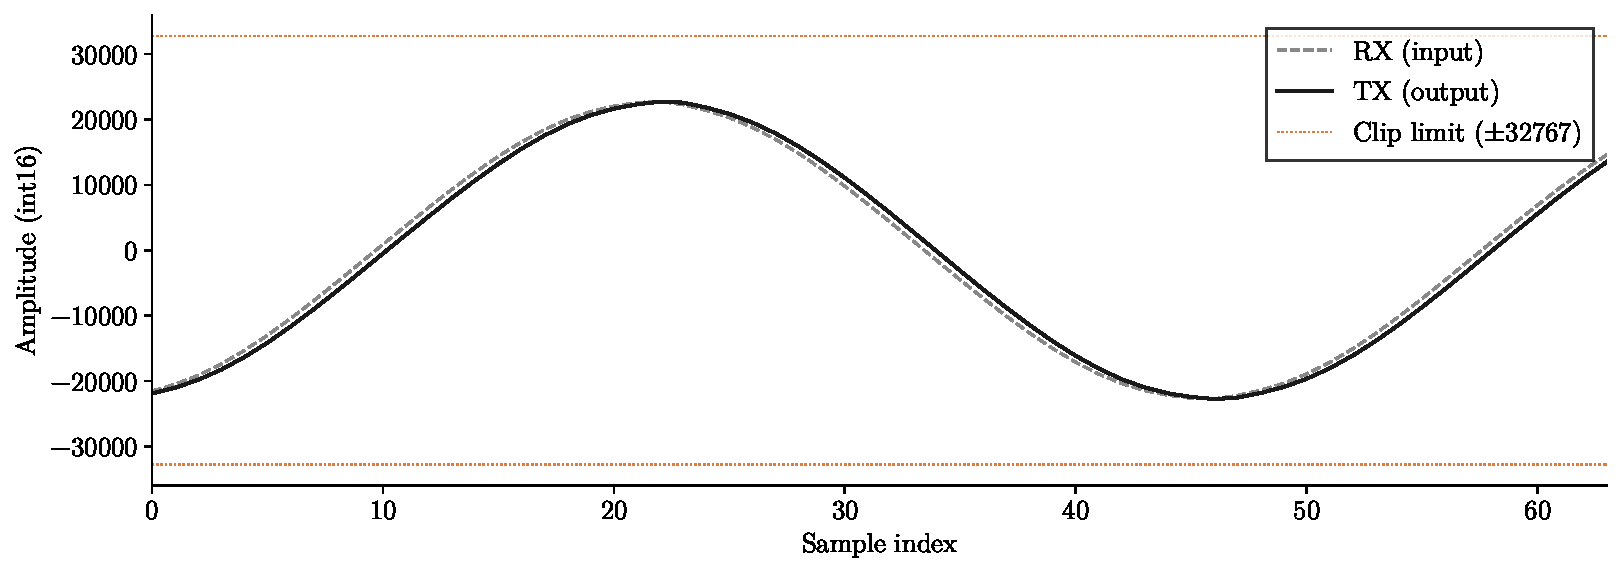
\includegraphics[width=0.9\textwidth]{../images/signal_tests/codec_loopback/fig_loopback_buf_10Vpp_sine_1kHz.pdf}
	\caption{RX/TX DMA buffer contents -- \SI{10}{V_{pp}} \qty{1}{kHz} sine wave.}
	\label{fig:loopback_buf}
\end{figure}

Both frequencies pass through the signal chain without observable distortion.
The output amplitude at \qty{1}{kHz} is \qty{7.68}{V_{pp}} versus \qty{7.20}{V_{pp}} at \qty{100}{Hz}, a difference of $20 \log_{10}(7.20 / 7.68) \approx \qty{-0.56}{dB}$.
This attenuation at \qty{100}{Hz} is consistent with the low-frequency rolloff identified in the frequency response measurement (Section~\ref{sec:frequency-response}, Figure~\ref{fig:frequency_response}).

The peak sample value at \qty{1}{kHz} corresponds to \qty{-3.2}{dBFS}, confirming \qty{3.2}{dB} of digital headroom at \SI{10}{V_{pp}} input -- the maximum standard Eurorack audio signal level (Section~\ref{sec:eurorack-fundamentals}).

The available headroom of \qty{3.2}{dB} is sufficient for the current implementation.
For future revisions, reducing the analog input gain would increase the digital headroom at the cost of a lower input signal level.
Since scaling up a signal in the digital domain is always possible — at the cost of increased
quantisation noise floor — a more conservative analog gain setting would give greater flexibility in the DSP processing chain.

\subsubsection{Frequency Response}
\label{sec:frequency-response}

\paragraph{Measurement Setup}

The frequency response of the analog signal path was measured using a logarithmic sine sweep from \qty{20}{Hz} to \qty{20}{kHz} generated in software and played back through the RME Fireface UFX\,II audio interface. 
The swept sine method was chosen as it provides a high signal-to-noise ratio across the full audio band and is robust against nonlinear distortion \cite[p.20]{massaraniTransferFunctionMeasurementSweeps2001}.

To remove the frequency response of the measurement chain itself — including the RME output and input stages, cables, and impedance interactions — a reference measurement was taken with the RME output connected directly to the RME input via a loopback cable. 
This reference response was then subtracted from the DUT measurement in the logarithmic domain, yielding the frequency response of the device under test alone:

\[
H_{\text{device}}(f) = H_{\text{DUT}}(f) - H_{\text{ref}}(f) \quad \text{[dB]}
\]

The DUT measurement was taken with the sweep signal routed through the module's 
analog frontend, AD conversion, firmware loopback, DA conversion, and analog 
output stage. The firmware was configured in loopback mode with unity gain and all 
DSP processing disabled.

Both measurements were performed at $f_s = \qty{48}{kHz}$ with a sweep duration 
of \qty{5}{s}, giving a frequency resolution of \qty{0.2}{Hz}. The resulting 
transfer function was smoothed with a simple moving average filter 
before plotting.

\paragraph{Results}



The high-pass filter at the ADC input is formed by the AC-coupling capacitor $C_3$ and 
the effective input impedance $R_{eq}$ of the TLV320AIC3204. In single-ended input mode, 
$R_{eq}$ depends on the programmed input resistor $R_{in}$ and the analog PGA gain $g$ 
(in linear terms) \cite{FAQTLV320AICCODECs2019}:

\[
R_{eq} = R_{in} \cdot \frac{1 + 2g}{1 + g}, \qquad
g = \frac{10000 \cdot 2^{\lfloor G/6 \rfloor}}{R_{in}}
\]

With $R_{in} = \SI{40}{\kilo\ohm}$ and a programmed PGA gain of $G = \SI{0}{\decibel}$, 
the linear gain evaluates to $g = 0.25$, giving:

\[
R_{eq} = \SI{40}{\kilo\ohm} \cdot \frac{1 + 0.5}{1 + 0.25} = \SI{48}{\kilo\ohm}
\]

The theoretical cutoff frequency is therefore:

\[
f_c = \frac{1}{2\pi \cdot R_{eq} \cdot C_3} 
= \frac{1}{2\pi \cdot \SI{48}{\kilo\ohm} \cdot \SI{2.2}{\micro\farad}} 
\approx \SI{1.5}{\Hz}
\]

This is well below the audible range.
However, the measured frequency response in Figure~\ref{fig:frequency_response} shows 
a high-pass rolloff with a \SI{-3}{\decibel} cutoff frequency of approximately \SI{37.6}{\Hz}.
The cause of this discrepancy has not yet been identified.
To isolate the source, individual frequency response measurements of the input and output stages should be conducted separately in a future revision.

\begin{figure}[H]
	\centering
	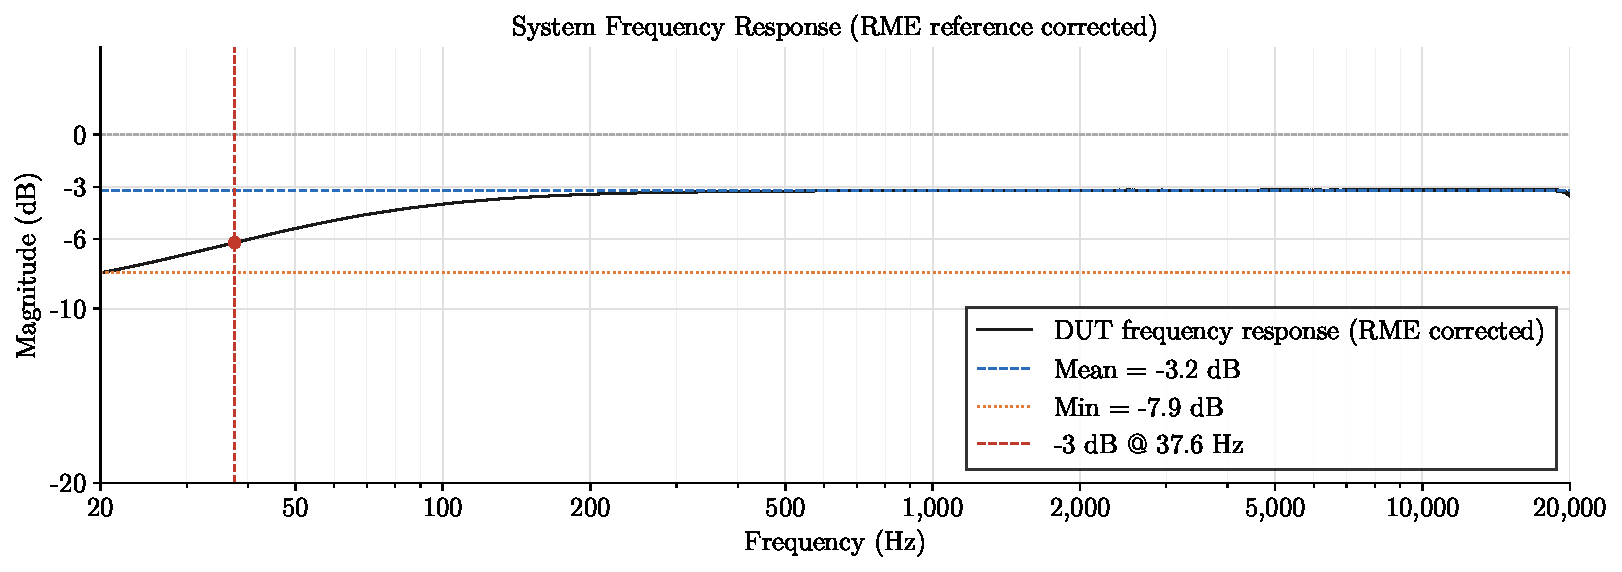
\includegraphics[width=1.0\textwidth]{../images/signal_tests/frequency_response/fig_frequency_response_aarebot_rme-corrected.pdf}
	\caption{Measured frequency response of the analog signal path, corrected for 
		the RME Fireface UFX\,II measurement chain response.}
	\label{fig:frequency_response}
\end{figure}

The measured passband shows a broadband attenuation of approximately \SI{-3.2}{\decibel}, 
which is expected given that the input stage attenuation exceeds the output stage gain. 
This offset can be compensated in software via PGA or digital gain adjustment

%\subsubsection{Noise and distortion measurements}
%
%\paragraph{Measurement Setup}
%The noise floor was measured by recording \qty{10}{\second} of silence at the module output with no input signal applied. 
%The spectrum was computed via FFT using a Hann window and normalised to amplitude spectral density in dBFS, correcting for the FFT bin width and window noise power bandwidth ($\text{NPB} = 1.50$) to ensure the result is independent of recording length \cite{FFTScalingNoise}:
%
%\[
%	\text{NF}[k] = 20 \log_{10}\!\left(
%	\frac{|S[k]|}{(n/2)\,\sqrt{\text{NPB}}}
%	\right)
%\]


